\documentclass{article}
\usepackage[T1]{fontenc}
\usepackage{lmodern}
\usepackage{amsmath}
\usepackage{amssymb}
\usepackage{tikz}
\usepackage[margin=1in]{geometry}


\title{Projet, MTH8414}
\author{Antoine Habib, Isaac Valin, Kinan Toutoungy}
\date{\today}

\begin{document}
\maketitle

\section*{Question 3 -- Sessions de recharge (programmation par contraintes)}

Fichiers : \texttt{Q3\_2.mzn} (questions 3.1 à 3.3) et \texttt{Q3\_4.mzn}. Toutes les résolutions utilisent une limite de 120~s.

\subsection*{3.1 Modèle}

\paragraph{Données}
\begin{itemize}
  \item $S$ : séjours ; $K = \{1, 2\}$ : types de chargeurs (1 = lent, 2 = rapide) ; $T = 48$ périodes.
  \item $a_s$ : première période du séjour $s$ ; $d_s$ : première période après le séjour ; $e_s$ : énergie à recharger (kWh).
  \item $P_k$ : puissance d'un chargeur de type $k$ (kW) ; $F_k$ : coût journalier d'un chargeur de type $k$.
  \item $h = 2$ : périodes par heure ; $D$ : prime de puissance par kW ; $G$ : limite du réseau (kW) ; $n_B$ : nombre de bus.
  \item $\delta_{sk} = e_s\,h / P_k$ : durée (en périodes) de la session du séjour $s$ sur un chargeur de type $k$. À $P_k$~kW, le bus reçoit $P_k/h$~kWh par période, donc il faut $e_s/(P_k/h)$ périodes.
\end{itemize}

\paragraph{Variables de décision} (aucune variable binaire)
\begin{itemize}
  \item $k_s \in K$ : type de chargeur de la session du séjour $s$.
  \item $t_s \in \{1, \dots, T\}$ : période de début de la session du séjour $s$.
  \item $N_k \in \{0, \dots, n_B\}$ : nombre de chargeurs de type $k$ installés (au plus un bus par chargeur, donc $n_B$ suffit).
  \item $P^{\max} \in \{0, \dots, G\}$ : puissance de pointe (kW). Son domaine impose la limite du réseau.
\end{itemize}
À partir du type choisi, on définit la durée $\Delta_s = \delta_{s,k_s}$ et la puissance $p_s = P_{k_s}$ de la session. Ce sont des contraintes \texttt{element} : un tableau de données indexé par une variable.

\paragraph{Contraintes}
\begin{enumerate}
  \item La session se déroule pendant le séjour :
  \[ t_s \geq a_s, \qquad t_s + \Delta_s \leq d_s \qquad \forall s \in S. \]
  La session occupe les périodes $t_s, \dots, t_s + \Delta_s - 1$ à la puissance $p_s$, sans interruption. Elle fournit donc $\Delta_s\,p_s/h = e_s$~kWh.
  \item Nombre de chargeurs de chaque type :
  \[ \texttt{cumulative}\big(t,\ \Delta,\ ([k_s = k])_{s \in S},\ N_k\big) \qquad \forall k \in K, \]
  où $[k_s = k]$ vaut 1 si la session $s$ utilise le type $k$ et 0 sinon.
  \item Puissance totale :
  \[ \texttt{cumulative}\big(t,\ \Delta,\ p,\ P^{\max}\big). \]
\end{enumerate}

\paragraph{Fonction objectif} (coût d'infrastructure)
\[ \min\ \sum_{k \in K} F_k\, N_k + D\, P^{\max}. \]
Les contraintes 2 et 3 imposent seulement $N_k \geq$ nombre de sessions simultanées de type $k$ et $P^{\max} \geq$ puissance totale à chaque période. Comme on minimise, $N_k$ et $P^{\max}$ prennent exactement ces maxima.

\paragraph{Contraintes globales}
\begin{itemize}
  \item \texttt{element} ($x = A[i]$ avec $i$ variable) : relie le type choisi $k_s$ à la durée et à la puissance de la session. Elle remplace les binaires « la session $s$ utilise le type $k$ » d'un modèle PLNE.
  \item \texttt{cumulative}$(t, \Delta, r, C)$ : à chaque période $\tau$, la somme des hauteurs $r_s$ des tâches en cours ($t_s \leq \tau < t_s + \Delta_s$) est au plus $C$. Avec la hauteur $[k_s = k]$, elle compte les sessions en cours sur le type $k$ ; avec la hauteur $p_s$, elle donne la puissance totale.
\end{itemize}

\subsection*{3.2 Résolution}

Sur \texttt{depot\_04.dzn}, Chuffed et Gecode prouvent l'optimum : 1 chargeur rapide et une pointe de 150~kW, soit $40 + 60 = 100$~\$.

Sur \texttt{depot\_12.dzn} :
\begin{center}\small\texttt{minizinc -{}-solver chuffed -I Project -s -{}-time-limit 120000 Q3/Q3\_2.mzn Project/depot\_12.dzn}\end{center}

\begin{center}
\begin{tabular}{lrr}
\hline
 & Chuffed & Gecode \\
\hline
Chargeurs (lents, rapides) & 0, 2 & 0, 2 \\
Pointe (kW) & 300 & 300 \\
Coût d'infrastructure & 200,00 \$ & 200,00 \$ \\
Optimalité prouvée & oui & oui \\
nodes & 20\,869 & 95 \\
failures & 11\,334 & 43 \\
solveTime (s) & 0,35 & 0,002 \\
\hline
\end{tabular}
\end{center}

Coût : 2 chargeurs rapides ($2 \times 40 = 80$~\$) et une prime de $0{,}40 \times 300 = 120$~\$.

\paragraph{Comparaison.} Les deux solveurs prouvent l'optimum en moins d'une seconde. Gecode fait une recherche en profondeur : il trouve vite une solution à 200~\$, puis \texttt{cumulative} élimine les combinaisons moins chères de $(N_1, N_2, P^{\max})$ en 43 échecs. Chuffed apprend une clause à chaque échec et redémarre souvent la recherche : il fait beaucoup plus de nœuds, mais chaque nœud coûte peu. Le problème est facile, car l'objectif ne dépend que de trois variables.

\subsection*{3.3 Diagramme de Gantt et comparaison avec la question 2.2}

\begin{figure}[h]
\centering
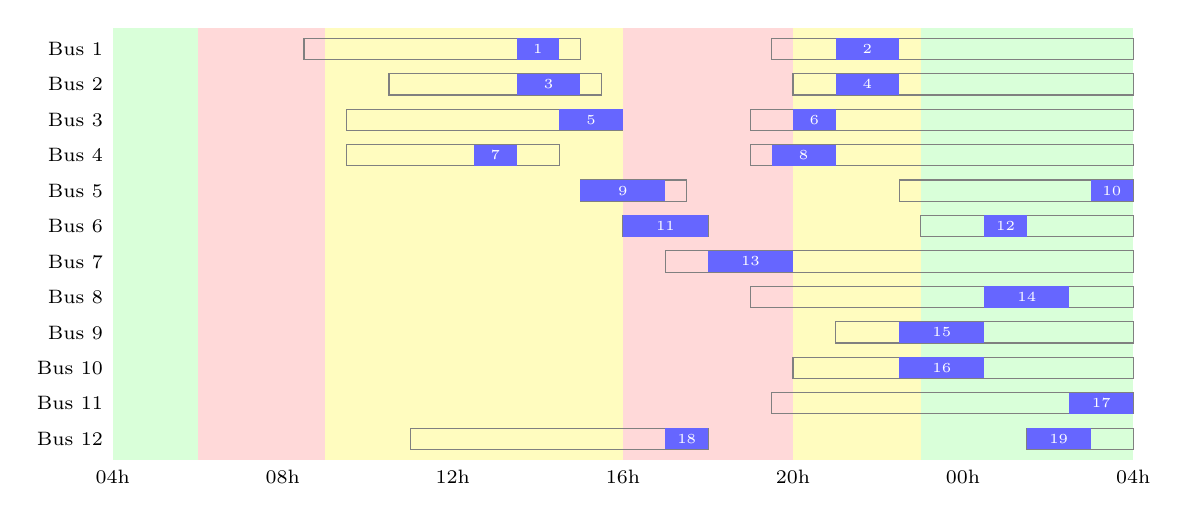
\begin{tikzpicture}[x=0.27cm, y=0.45cm]
  % Fond : prix de l'energie (vert 6, rouge 16, jaune 9 cents/kWh) ; la periode t va de t-1 a t
  \foreach \a/\b/\c in {0/4/green!15, 4/10/red!15, 10/24/yellow!25, 24/32/red!15, 32/38/yellow!25, 38/48/green!15}
    \fill[\c] (\a, 0.4) rectangle (\b, 12.6);
  % Sejours au depot (bus/arrivee/depart)
  \foreach \bus/\a/\d in {1/10/23, 1/32/49, 2/14/24, 2/33/49, 3/12/25, 3/31/49, 4/12/22, 4/31/49, 5/23/28, 5/38/49,
                         6/25/29, 6/39/49, 7/27/49, 8/31/49, 9/35/49, 10/33/49, 11/32/49, 12/15/29, 12/44/49}
    \draw[gray] (\a-1, 13-\bus-0.3) rectangle (\d-1, 13-\bus+0.3);
  % Sessions sur chargeur rapide (bus/debut/fin exclue/sejour)
  \foreach \bus/\t/\f/\s in {1/20/22/1, 1/35/38/2, 2/20/23/3, 2/35/38/4, 3/22/25/5, 3/33/35/6, 4/18/20/7, 4/32/35/8,
                             5/23/27/9, 5/47/49/10, 6/25/29/11, 6/42/44/12, 7/29/33/13, 8/42/46/14, 9/38/42/15,
                             10/38/42/16, 11/46/49/17, 12/27/29/18, 12/44/47/19}
    \fill[blue!60] (\t-1, 13-\bus-0.3) rectangle node[white, font=\tiny] {\s} (\f-1, 13-\bus+0.3);
  % Axes
  \foreach \bus in {1,...,12} \node[left, font=\scriptsize] at (0, 13-\bus) {Bus \bus};
  \foreach \t/\l in {0/04h, 8/08h, 16/12h, 24/16h, 32/20h, 40/00h, 48/04h}
    \node[below, font=\scriptsize] at (\t, 0.4) {\l};
\end{tikzpicture}
\caption{Solution de la question 3.2 (Chuffed). Cadre gris : séjour au dépôt ; bleu : session sur un chargeur rapide (numéro du séjour). Fond : prix de l'énergie (vert 6~¢, jaune 9~¢, rouge 16~¢/kWh).}
\end{figure}

\begin{center}
\begin{tabular}{lrr}
\hline
 & Question 2.2 (PLNE) & Question 3.2 (PC) \\
\hline
Chargeurs (lents, rapides) & 1, 2 & 0, 2 \\
Pointe (kW) & 350 & 300 \\
Infrastructure (chargeurs + prime) & 235,00 \$ & 200,00 \$ \\
Énergie & 362,00 \$ & 408,00 \$ \\
Infrastructure + énergie & 597,00 \$ & 608,00 \$ \\
\hline
\end{tabular}
\end{center}

\paragraph{Coût de l'énergie de la solution 3.2.} Il vaut 408,00~\$ (affiché par \texttt{Q3\_2.mzn}) :
\[ \sum_{s \in S} \frac{p_s}{h} \sum_{u=t_s}^{t_s+\Delta_s-1} \pi_u, \]
c'est-à-dire, pour chaque session, l'énergie reçue par période ($p_s/h$~kWh) multipliée par le prix $\pi_u$ de chaque période couverte. Ce coût n'est pas optimisé ici : Gecode trouve une autre solution à 200~\$ dont l'énergie coûte 415,50~\$. En ajoutant les 19 branchements (57~\$), le coût journalier complet de notre solution est $80 + 120 + 408 + 57 = 665{,}00$~\$ (solution détaillée en annexe).

\paragraph{Le paradoxe apparent.} Un plan par sessions est un cas particulier d'un plan de la partie 2 (on recharge à $P_{k_s}$ pendant la session et à 0 ailleurs). Le modèle de la partie 2 est donc une relaxation de celui de la partie 3, et il ne peut pas être plus cher \emph{pour le même objectif}. Mais les objectifs diffèrent : la question 2.2 minimise infrastructure \emph{plus} énergie, alors que la question 3.2 minimise seulement l'infrastructure. La question 2.2 accepte de payer 35~\$ de plus en infrastructure (un chargeur lent et 50~kW de pointe) pour recharger davantage aux heures à 6 et 9~¢ et économiser 46~\$ d'énergie. Avec l'objectif de la question 2.2, le plan 3.2 coûte $200 + 408 = 608 \geq 597$~\$ : la relaxation est bien respectée.

\subsection*{3.4 Coût journalier complet}

\paragraph{a) Coût de l'énergie d'une session.} On calcule à l'avance, pour chaque séjour $s$, type $k$ et début $t$,
\[ \gamma_{skt} = \frac{P_k}{h} \sum_{u=t}^{t+\delta_{sk}-1} \pi_u \]
(\texttt{coutSession}), le coût de la session si elle commence à $t$. On met $\gamma_{skt} = 0$ si la session déborde de la journée (ce début est interdit par la contrainte 1). Une contrainte \texttt{element} à deux indices variables choisit l'entrée du type et du début retenus :
\[ g_s = \gamma_{s,\,k_s,\,t_s} \quad \forall s \in S, \qquad
   \min\ \sum_{k} F_k N_k + D\,P^{\max} + \sum_{s} g_s + 3\,\$ \times |S|. \]
Chaque session demande exactement un branchement : ce coût est constant ($3 \times 19 = 57$~\$).

\paragraph{b) Résultats} (\texttt{Q3\_4.mzn}, \texttt{depot\_12.dzn}, 120~s) :

\begin{center}
\begin{tabular}{lrr}
\hline
 & Chuffed & Gecode \\
\hline
Meilleur coût total & 693,80 \$ & 654,50 \$ \\
Chargeurs (lents, rapides) & 1, 2 & 0, 2 \\
Pointe (kW) & 417 & 300 \\
Énergie & 375,00 \$ & 397,50 \$ \\
nodes & 3\,501\,756 & 6\,617\,045 \\
failures & 2\,981\,055 & 3\,308\,511 \\
Optimalité prouvée & non & non \\
\hline
\end{tabular}
\end{center}

Gecode garde l'infrastructure de la question 3.2 (0 lent, 2 rapides, 300~kW) et réduit l'énergie de 408,00 à 397,50~\$, soit 654,50~\$ au total. La meilleure solution de Chuffed paie une prime sur 417~kW, alors que ses sessions n'appellent jamais plus de 350~kW : en 120~s, Chuffed n'a même pas ramené la pointe à sa valeur minimale.

Contrairement à la question 3.2, aucun solveur ne prouve l'optimum. À la question 3.2, l'objectif ne dépend que de $N_1$, $N_2$ et $P^{\max}$ : une fois 200~\$ trouvé, il reste peu de combinaisons moins chères à réfuter. Ici, l'objectif dépend aussi du début de chacune des 19 sessions. La borne inférieure sur $\sum_s g_s$ obtenue par propagation place chaque session à son meilleur moment comme si elle était seule, sans tenir compte des chargeurs ni de la pointe. Cette borne est faible, et la recherche doit énumérer un très grand nombre de débuts.

\section*{Annexe -- Solution complète de la question 3.3 (\texttt{depot\_12})}

Comme la question 3.5 n'est pas évaluée, on donne la solution de la question 3.3 (\texttt{Q3\_2.mzn}, Chuffed, celle du diagramme de Gantt) : 0 chargeur lent, 2 chargeurs rapides (80~\$), pointe de 300~kW (prime 120~\$), 19 branchements (57~\$), énergie 408,00~\$, coût total 665,00~\$. Chaque ligne est la session d'un séjour, sur un chargeur rapide (150~kW), sans interruption. La période 1 commence à 04:00. Le coût est la somme des prix des périodes occupées multipliée par 75~kWh.

\begin{center}
\begin{tabular}{rrlccrrr}
\hline
Bus & Séjour & Chargeur & Début & Fin & Périodes & Énergie (kWh) & Coût (\$) \\
\hline
1 & 1 & rapide & 13:30 & 14:30 & 20--21 & 150 & 13,50 \\
1 & 2 & rapide & 21:00 & 22:30 & 35--37 & 225 & 20,25 \\
2 & 3 & rapide & 13:30 & 15:00 & 20--22 & 225 & 20,25 \\
2 & 4 & rapide & 21:00 & 22:30 & 35--37 & 225 & 20,25 \\
3 & 5 & rapide & 14:30 & 16:00 & 22--24 & 225 & 20,25 \\
3 & 6 & rapide & 20:00 & 21:00 & 33--34 & 150 & 13,50 \\
4 & 7 & rapide & 12:30 & 13:30 & 18--19 & 150 & 13,50 \\
4 & 8 & rapide & 19:30 & 21:00 & 32--34 & 225 & 25,50 \\
5 & 9 & rapide & 15:00 & 17:00 & 23--26 & 300 & 37,50 \\
5 & 10 & rapide & 03:00 & 04:00 & 47--48 & 150 & 9,00 \\
6 & 11 & rapide & 16:00 & 18:00 & 25--28 & 300 & 48,00 \\
6 & 12 & rapide & 00:30 & 01:30 & 42--43 & 150 & 9,00 \\
7 & 13 & rapide & 18:00 & 20:00 & 29--32 & 300 & 48,00 \\
8 & 14 & rapide & 00:30 & 02:30 & 42--45 & 300 & 18,00 \\
9 & 15 & rapide & 22:30 & 00:30 & 38--41 & 300 & 20,25 \\
10 & 16 & rapide & 22:30 & 00:30 & 38--41 & 300 & 20,25 \\
11 & 17 & rapide & 02:30 & 04:00 & 46--48 & 225 & 13,50 \\
12 & 18 & rapide & 17:00 & 18:00 & 27--28 & 150 & 24,00 \\
12 & 19 & rapide & 01:30 & 03:00 & 44--46 & 225 & 13,50 \\
\hline
\multicolumn{7}{r}{Total énergie} & 408,00 \\
\hline
\end{tabular}
\end{center}

\end{document}
